\documentclass[tikz,border=2pt]{standalone}
\usepackage{amsmath}
\usetikzlibrary{arrows.meta}
\begin{document}
% Prisoner's Dilemma: in each column player 1 gains by moving from M to F (-2 -> -1, -5 -> -4),
% in each row player 2 gains by moving from M to F, so F is strictly dominant for both and
% (F,F) with (-4,-4) is the strictly dominant strategy equilibrium.
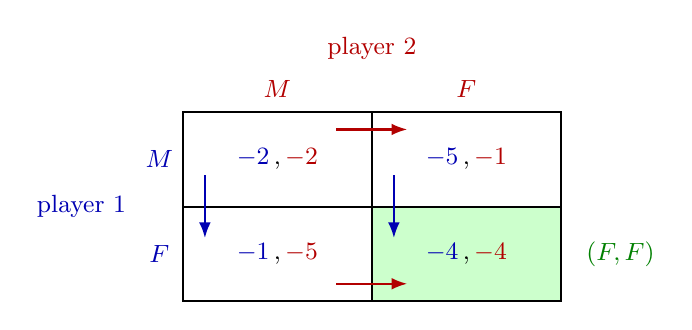
\begin{tikzpicture}[font=\small, >={Latex[length=2mm]}]
  \def\w{2.4} \def\h{1.2}
  \fill[green!20] (\w,-\h) rectangle (2*\w,0);
  \draw[thick] (0,-\h) rectangle (2*\w,\h);
  \draw[thick] (\w,-\h) -- (\w,\h);
  \draw[thick] (0,0) -- (2*\w,0);
  % strategy labels
  \node[red!70!black] at (0.5*\w,\h+0.3) {$M$};
  \node[red!70!black] at (1.5*\w,\h+0.3) {$F$};
  \node[blue!70!black] at (-0.3,0.5*\h) {$M$};
  \node[blue!70!black] at (-0.3,-0.5*\h) {$F$};
  \node[red!70!black, anchor=south] at (\w,\h+0.55) {player 2};
  \node[blue!70!black, anchor=east] at (-0.6,0) {player 1};
  % payoffs
  \node at (0.5*\w,0.5*\h) {\textcolor{blue!70!black}{$-2$}\,,\,\textcolor{red!70!black}{$-2$}};
  \node at (1.5*\w,0.5*\h) {\textcolor{blue!70!black}{$-5$}\,,\,\textcolor{red!70!black}{$-1$}};
  \node at (0.5*\w,-0.5*\h) {\textcolor{blue!70!black}{$-1$}\,,\,\textcolor{red!70!black}{$-5$}};
  \node at (1.5*\w,-0.5*\h) {\textcolor{blue!70!black}{$-4$}\,,\,\textcolor{red!70!black}{$-4$}};
  % player 1: F better in every column
  \foreach \c in {0,1} \draw[->, thick, blue!70!black] (\c*\w+0.28,0.4) -- (\c*\w+0.28,-0.4);
  % player 2: F better in every row
  \foreach \r in {0,1} \draw[->, thick, red!70!black] (\w-0.45,\h-0.22-\r*1.96) -- (\w+0.45,\h-0.22-\r*1.96);
  \node[green!50!black, anchor=west] at (2*\w+0.2,-0.5*\h) {$(F,F)$};
\end{tikzpicture}
\end{document}
